\documentclass[tikz]{standalone}

\usepackage{pgfplots,mathtools}
\pgfplotsset{compat=newest}

\begin{document}
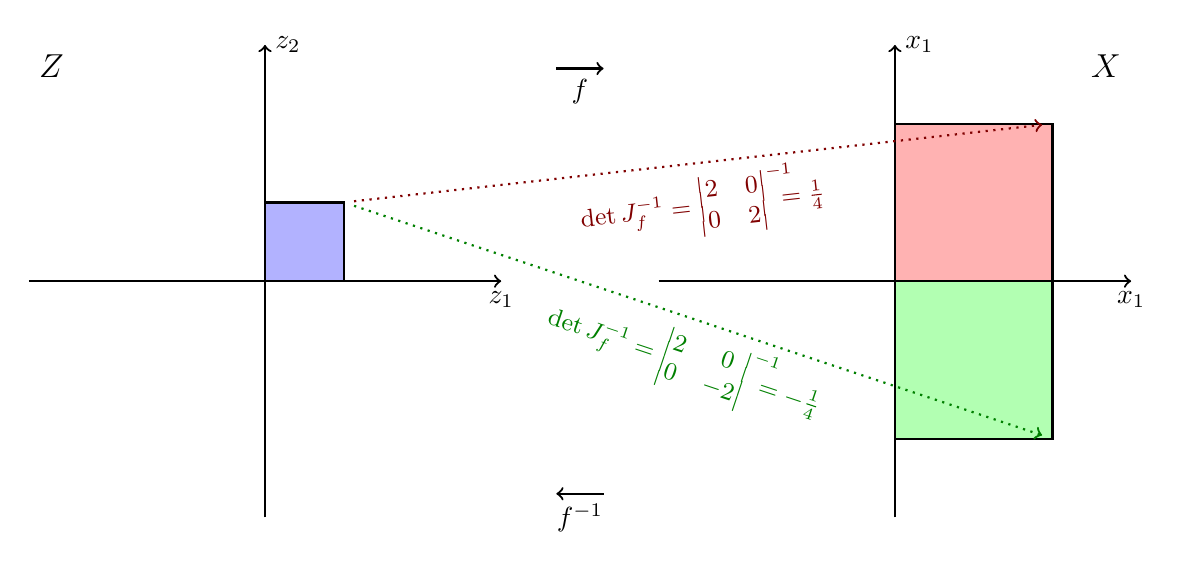
\begin{tikzpicture}[thick]
  \draw[->] (-3,0) -- (3,0) node[below] {$z_1$};
  \draw[->] (0,-3) -- (0,3) node[right] {$z_2$};
  \draw[fill=blue!30] (0,0) rectangle (1,1) node (z1) {};
  \node[below right,font=\large] at (-3,3) {$Z$};

  \begin{scope}[xshift=4cm]
    \draw[->] (-0.3,2.7) -- node[midway,below] {$f$} (0.3,2.7);
    \draw[<-] (-0.3,-2.7) -- node[midway,below] {$f^{-1}$} (0.3,-2.7);
  \end{scope}

  \begin{scope}[xshift=8cm]
    \draw[->] (-3,0) -- (3,0) node[below] {$x_1$};
    \draw[->] (0,-3) -- (0,3) node[right] {$x_1$};
    \draw[fill=red!30] (0,0) rectangle (2,2) node (x1) {};
    \draw[fill=green!30] (0,0) rectangle (2,-2) node (x2) {};
    \node[below left,font=\large] at (3,3) {$X$};
  \end{scope}

  \draw[->,dotted,red!50!black] (z1) -- node[midway,below,sloped,font=\small] {$\det J_f^{-1} = \begin{vmatrix} 2 & 0 \\ 0 & 2 \end{vmatrix}^{-1} \mkern-15mu = \frac 1 4$} (x1);
  \draw[->,dotted,green!50!black] (z1) -- node[midway,below,sloped,font=\small] {$\det J_f^{-1} = \begin{vmatrix} 2 & 0 \\ 0 & -2 \end{vmatrix}^{-1} \mkern-15mu = -\frac 1 4$} (x2);
\end{tikzpicture}
\end{document}
